\begin{figure}[H] % Để canh giữa và thêm chú thích
    \centering % Canh giữa hình
    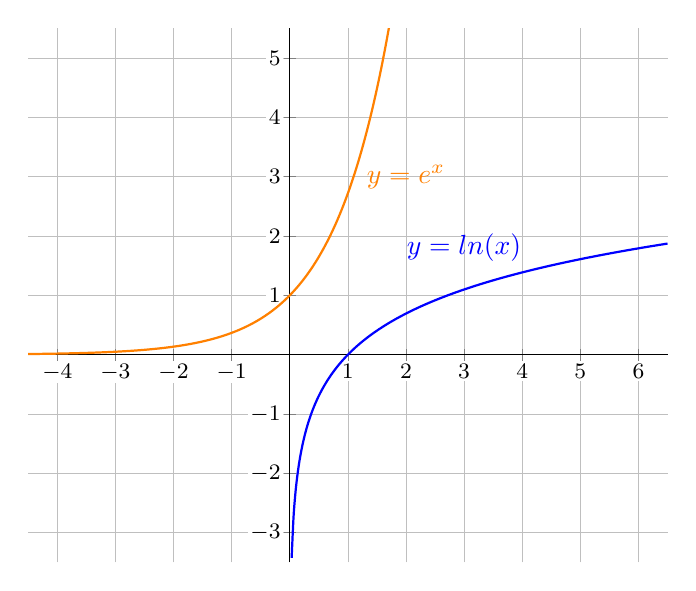
\begin{tikzpicture}
        \begin{axis}[
            width=0.8\textwidth,
            % height=12cm,
            axis lines=middle,
            grid=major,
            grid style={line width=.1pt, draw=gray!20},
            major grid style={line width=.2pt,draw=gray!50},
            xmin=-4.5, xmax=6.5,
            ymin=-3.5, ymax=5.5,
            xtick={-4, -3, -2, -1, 0, 1, 2, 3, 4, 5, 6},
            ytick={-3, -2, -1, 0, 1, 2, 3, 4, 5, 6},
            ticklabel style={font=\footnotesize, fill=white, inner sep=1pt},
            axis line style={-},
            smooth,
            no marks,
            samples=200,
        ]

        % Vẽ đồ thị y = e^x
        \addplot[orange, thick, domain=-5:1.85] {exp(x)};
        \node[orange] at (axis cs:2, 3) {$y=e^x$};

        % Vẽ đồ thị y = ln(x)
        \addplot[blue, thick, domain=0:6.5] {ln(x)};
        \node[blue] at (axis cs:3, 1.8) {$y=ln(x)$};

        \end{axis}
    \end{tikzpicture}
    \caption{Đồ thị các hàm số $y = e^x$ và $y = ln(x)$.} % Thêm chú thích cho hình (tùy chọn)
    \label{fig:plot_e^x_ln(x)} % Thêm nhãn để tham chiếu (tùy chọn)
\end{figure}